\documentclass[11pt,t]{beamer}
%% Language and font encodings
\usepackage[english]{babel}
\usepackage[utf8x]{inputenc}
\usepackage[T1]{fontenc}

\usepackage{helvet}

%% Sets page size and margins
\usepackage[letterpaper,top=3cm,bottom=2cm,left=3cm,right=3cm,marginparwidth=1.75cm]{geometry}

%% Useful packages
\usepackage{amsmath}
\usepackage{graphicx}
\usepackage{tcolorbox}
\usepackage{amssymb}
\usepackage{amsthm}
\usepackage{lastpage}
\usepackage{accents}
\usepackage{multicol}

% For better list numbering
\usepackage[shortlabels]{enumitem}

% Font
% \usepackage{tgbonum}


% Tikz
\usepackage{tikz}

\usetikzlibrary{calc,fit,shapes.misc,backgrounds}
\usepackage{pgfplots}
\pgfplotsset{compat = newest}
\usetikzlibrary{positioning, arrows.meta}
\usepgfplotslibrary{fillbetween}

% Headers
\usepackage{fancyhdr}
\pagestyle{fancy}

% Store \@title as \thetitle
\makeatletter
\let\thetitle\@title
\makeatother

\fancyhf{}
\lhead{\fontfamily{qbk}\fontsize{10}{11}\selectfont ECON 3070}
\rhead{\fontfamily{qbk}\fontsize{10}{11}\selectfont \thetitle}
\rfoot{\fontfamily{qbk}\fontsize{10}{11}\selectfont \thepage}


% Sections and Subsections

% define colors
\definecolor{buff-gold}{HTML}{CFB87C}
\definecolor{buff-grey}{HTML}{565A5C}
% custom tcolorbox
\tcbset{colframe=buff-gold, colback=white!100!black}

% new page per section
\usepackage{titlesec}
\newcommand{\sectionbreak}{\clearpage}
% change style of section
\usepackage{sectsty}
\sectionfont{\color{buff-gold} \fontfamily{qbk}\selectfont}
\subsectionfont{\color{buff-grey} \fontfamily{qbk}\selectfont}


\author{Kyle Butts}
\title{Lecture 9 - Perfect Competition}
\subtitle{ECON 3070 - Intermediate Microeconomic Theory}

\begin{document}

\begin{frame}
  \titlepage
\end{frame}

\begin{frame}{Overview}
  In this chapter, we will:

  \begin{itemize}
    \item Define a perfectly competitive market.
    
    \item Discuss the difference between economic profit and accounting profit.
    
    \item Learn how to calculate a firm's optimal input combination for profit maximization.
    
    \item Consider both short-run and long-run profit-maximization
  \end{itemize}
\end{frame}

\begin{frame}{Perfectly Competitive Markets}
  Perfectly competitive markets have 4 defining characteristics:

  \begin{enumerate}
    \item Fragmented market - many buyers and sellers
    
    \item Undifferentiated products (e.g. oil, corn, soybeans).
    
    \item Consumers have perfect information about prices of all sellers
    
    \item Equal access to resources - same technology, access to same inputs
  \end{enumerate}
\end{frame}

\begin{frame}{Perfectly Competitive Markets}
  These characteristics have 3 implications:
  \bigskip

  \begin{enumerate}
    \item Buyers and sellers are price takers
    
    \item Law of one price - demand is perfectly elastic
    
    \item Free entry and exit - If market is profitable, firms enter. If unprofitable, firms exit.
  \end{enumerate}

  \bigskip
  This final implication implies that profits equal zero
\end{frame}

\begin{frame}{Economic \& Accounting Profits}
  What do I mean by zero profits? Why would anyone start a company in a perfectly competitive market if they're guaranteec to make 0 profits!!

  \bigskip\pause
  Remember that economic costs = explicit costs + implicit costs (such as the opportunity cost of not working a job)

  \begin{itemize}
    \item \textbf{Economic profit} = Sales Revenue - Economic Costs
    
    \item \textbf{Accounting profit} = Sales Revenue - Accounting Costs
  \end{itemize}


  \bigskip
  \emph{When we discuss profit maximization, we mean economic profit.}
\end{frame}

\begin{frame}{\bgCoral{Try It Yourself}}
  Suppose that Tom, a lawyer quits his job to start a lawn care company. Before he quit, the lawyer was earning \$120,000 per year (which he could return to at any time). With the lawn care company, Tom expects his revenue to be \$300,000 per year. He expects his annual cost of wages for workers to be \$80,000, and additional operating costs to be \$20,000. Additionally, Tom invested \$80,000 in equipment, money which he could have otherwise invested in the stock market, with a return of \$5,000 per year. Find Tom's economic profit.
\end{frame}

\begin{frame}{Profit Maximization}
  Remember that a firm's profit function looks like
  $$
    \pi = P * Q - TC(Q,w,r)
  $$
  where $P * Q$ is equal to total revenue, $TR(Q) = PQ$.

  \begin{itemize}
    \item $TC(Q,w,r)$ is the total cost function that we looked at in chapters 7 and 8.
    
    \item Because the firm is a price taker, $P$ doesn't depend on how many units the firm sells.
  \end{itemize}
\end{frame}

\begin{frame}{Profit Maximization}
  A profit-maximizing perfectly competitive firm chooses the quantity $Q$ which maximizes profit.

  \bigskip
  In other words, the firm's problem is
  $$
    \max_Q \pi(Q) = PQ-TC(Q,w,r)
  $$

  \bigskip\pause
  If we take the partial derivative of this equation with respect to Q and set it to zero, we find the quantity that maximizes profit.
  $$
    P-\frac{\partial TC(Q,w,r)}{\partial Q} = 0  \Rightarrow P = MC(Q,w,r)
  $$
\end{frame}

\begin{frame}{Profit Maximization}
  In words, the firm will produce output until the revenue it receives from an additional unit ($P$) equals the marginal cost of producing that unit ($MC(Q)$).

  \begin{itemize}
    \item The revenue that it receives from an additional unit of output is called \textbf{marginal revenue}.
    
    \item That is, $Q$ is chosen such that $P = MR = MC$.
  \end{itemize}
\end{frame}

\begin{frame}{Profit Maximization}
  Here's the intuition: After some point, MC is increasing. As long as a firm can sell a unit for more than it's marginal cost, $P > MC(Q)$, it should keep selling more units.

  \bigskip\pause
  Eventually, marginal cost will rise enough that price is below marginal cost.

  \begin{itemize}
    \item At that point, a firm would lose money on each additional unit sold.
  \end{itemize}

  \bigskip \pause
  $\implies$ profit is maximized where $P = MC(Q)$.
\end{frame}

\begin{frame}
  \begin{figure}
    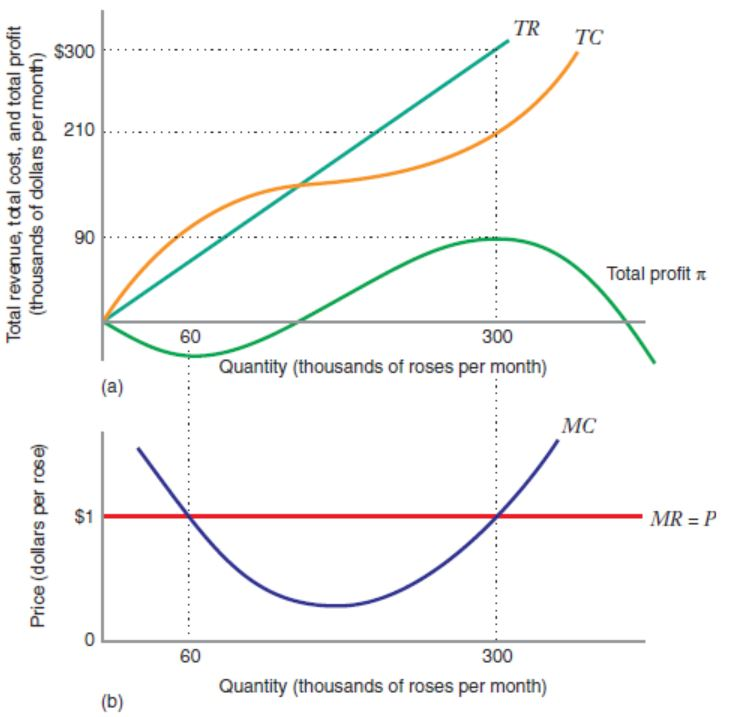
\includegraphics[width=260px]{figures/fig9_1.jpg}
  \end{figure}
\end{frame}

\begin{frame}{Profit Maximization}
  Once you have found the marginal cost function, all you need to do is solve $P = MC(Q,w,r)$ for $Q$.
  
  Either you will be given
  \begin{enumerate}
    \item $TC(Q)$, or
    
    \item will have to derive it from a production function $Q(K, L)$
  \end{enumerate}
\end{frame}

\begin{frame}{Example}
  Suppose a firm's total cost function is given by
  $$
    TC(Q,w,r) = 2wQ^2+8r
  $$

  \bigskip
  The firm's profit maximizing quantity of output must satisfy $P = MC$:
  \pause
  $$
    MC(Q,w,r) = \frac{\partial TC(Q,w,r)}{\partial Q} = 4wQ
  $$

  \bigskip
  Solving for Q:
  \pause
  $$
    P=4wQ  \Rightarrow Q^* = \frac{P}{4w}
  $$
\end{frame}

\begin{frame}{Profit Maximization}
  Now that we know $Q^*(P,r,w)$, we can plug that back into our conditional input demand functions for capital and labor and find our \textbf{unconditional input demand functions}.

  \begin{itemize}
    \item These functions do not condition on a given level of quantity $\bar{Q}$.
    
    \item Instead, they implicitly reflect how Q will change as P changes, in order to maximize profit.
  \end{itemize}
\end{frame}

\begin{frame}{Profit Maximization}
  Another way that we can find the firm's profit maximizing output quantity is by writing total cost as a function of L and K:
  $$
    Q = f(K,L) \text{ and } TC(Q,w,r) = wL + rK
  $$ 
  
  Plugging those into the firm's profit function, the firm's problem then becomes:
  $$
    \max_{L,K} \pi = P*f(K,L) - wL - rK
  $$
\end{frame}

\begin{frame}{Profit Maximization}
  $$
    \max_{L,K} \pi = P*f(K,L) - wL - rK
  $$
  
  Again using unconstrained optimization, we can find the two first-order conditions:
  \begin{align*}
    \frac{\partial \pi}{\partial L} & =P \frac{\partial f}{\partial L} - w = 0 \Rightarrow P = \frac{w}{MP_L} \\
    \frac{\partial \pi}{\partial K} & =P \frac{\partial f}{\partial K} - r = 0 \Rightarrow P = \frac{r}{MP_k}
  \end{align*}
\end{frame}

\begin{frame}{Profit Maximization}
  If we combine the two first-order conditions, we get the following \textbf{optimality condition} for price maximization:
  $$
    P = \frac{w}{MP_L} = \frac{r}{MP_k}
  $$
  The second part of this looks a lot like our optimality condition for cost minimization.

  \bigskip
  That's because maximizing profit requires producing at the lowest cost.
\end{frame}

\begin{frame}{Profit Maximization}
  If we rearrange our first-order conditions in a different way:
  $$
    P * MP_L = w \text{ and } P * MP_K = r
  $$
  This tells us that the cost of an additional unit of capital or labor should equal the revenue that it generates.

  \bigskip
  At the optimal output level the price of the output good should equal the amount of money it costs to produce the last unit with either labor or capital. That is,
  $$
    P = MC(Q)
  $$
\end{frame}


\begin{frame}{\bgCoral{Example}}
  Suppose that a firm has the production function $Q(K,L) = 20K-K^2 + 16L-L^2$ with $MP_L = 16-2L$ and $MP_K = 20-2K$.

  \bigskip
  Our optimality condition says that
  $$
    P = \frac{w}{16 - 2L} \text{ and } P = \frac{r}{20 - 2K}
  $$

\end{frame}

\begin{frame}{\bgCoral{Example}}
  $$
    P = \frac{w}{16 - 2L} \text{ and } P = \frac{r}{20 - 2K}
  $$

  \bigskip
  We can solve for $K$ in the second equation, and find that
  $$
    20-2K=\frac{r}{P} \text{ or }  K^*(P,w,r) = 10- \frac{r}{2P}
  $$

  \pause
  Doing the same with the first equation, we find that
  $$
    16-2L = \frac{w}{P} \text{ or } L^*(P,w,r) = 8 - \frac{w}{2P}
  $$
\end{frame}

\begin{frame}{Profit Maximization}
  Once we've found the unconditional input demand curves, we can now solve for the optimal production function: $Q^*(P,w,r)$.

  That is;
  $$
    Q^*(P,w,r) = Q\big( K^*(P,w,r), L^*(P,w,r) \big)
  $$
\end{frame}

\begin{frame}{\bgCoral{Try It Yourself}}
  Suppose that a profit-maximizing firm has the production function $Q(K,L) = 30K-\frac{1}{2}K^2+40L-\frac{1}{2}L^2$, with $MP_L = 40-L$ and $MP_K=30-K$.  Find the firm's unconditional labor demand function.
\end{frame}

\frame

\begin{frame}{Short-Run Profit Maximization}
  Suppose that $K$ is fixed ($K = \bar{K}$) in the short run.

  Can solve profit maximization problem with one variable input.
  $$
    \max_{L}\pi(P,r,w) = PQ(L,\bar{K}) - wL - r\bar{K}
  $$
  FOC: 
  
  $$
    P * \frac{\partial Q(L, \bar{K})}{\partial L} - W = 0 \Rightarrow P = \frac{w}{MP_L} \only<2>{\Rightarrow P = SMC(Q,w)}
  $$

  \bigskip
  \only<2>{No cost minimization condition, because there is only one way to produce $Q$ units.}
\end{frame}

\begin{frame}{Deriving the Firm's Supply Curve}
  The solution to the firm's problem gives us the firm's supply function:
  $$
    Q^*(P,w,r)
  $$

  \bigskip
  If $w$ and $r$ are fixed, can plot firm's supply curve in P-Q space.

  \bigskip\pause
  Recall the profit maximizing condition under perfect competition in the short run: $P = SMC(Q)$

  \begin{itemize}
    \item Inverse supply curve is the short-run marginal cost curve 
    
    (you give me $Q$, I give you $SMC(Q)$)
  \end{itemize}
\end{frame}

\begin{frame}{Deriving the Firm's Supply Curve}
  \textbf{There is an exception though.}

  \bigskip\pause
  Suppose the firm has large fixed costs that could be recovered if firm sets $Q = 0$ (e.g. electricity costs)

  \smallskip
  Perhaps even at profit-maximizing quantity, profits do not offset total fixed costs (TFC).
  \begin{itemize}
    \item Then $Q=0$ is optimal.
    \item Will occur if market price of final good is low enough.
  \end{itemize}
\end{frame}

\begin{frame}{Deriving the Firm's Supply Curve}
  If firm is making positive profit when $Q > 0$, must be making positive \textit{per-unit} profit

  \begin{itemize}
    \item Because all units sell at price $P$, that means that average variable cost is below the price $P > ATC(Q)$.
    
    \item If $P < \min(ATC(Q))$, firm will produce $Q=0$ in the long-run. 
  \end{itemize}
  
  \bigskip\pause
  The price at which $P = \min(ATC(Q))$ is called the \textbf{break-even price}
\end{frame}

\begin{frame}{Deriving the Firm's Supply Curve}
  In the short-run, the fixed costs are already paid for (sunk costs). Therefore, `short-run profit' is the difference between market price and \emph{average variable cost}. 

  The reason is if price is above $AVC$, then you can pay off some of your sunk costs. 

  \begin{itemize}
    \item Because all units sell at price $P$, that means that average variable cost is below the price $P > AVC(Q)$.
    
    \item If $P < \min(AVC(Q))$, firm will produce $Q=0$ in the short-run.
  \end{itemize}
  
  \bigskip\pause
  The price at which $P = \min(AVC(Q))$ is called the \textbf{shut-down price}
\end{frame}

\begin{frame}{Deriving the Firm's Supply Curve}
  \begin{figure}
    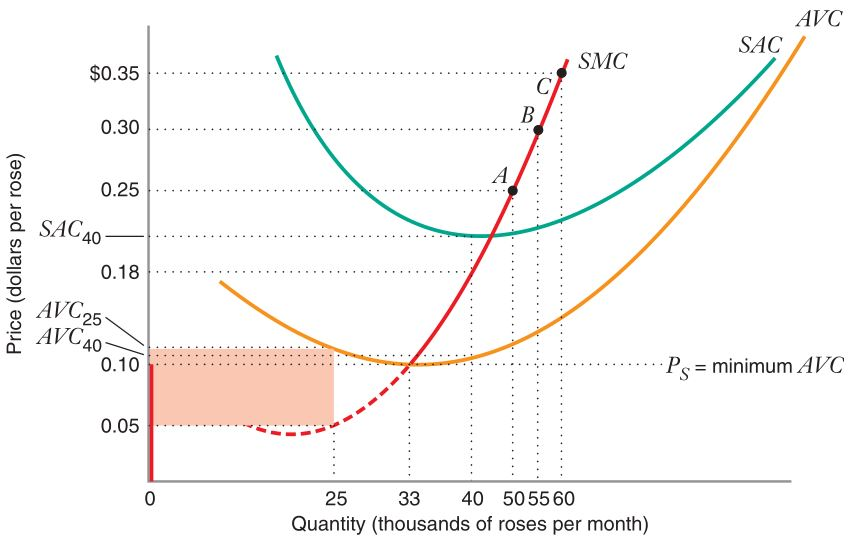
\includegraphics[width=280px]{figures/fig9_2.jpg}
  \end{figure}
\end{frame}

\begin{frame}{Short-Run Market Supply}
  Once we have each firm's supply curve, we can find the market supply curve. The market supply curve tells us the quantity supplied by \textit{all firms} at any given price.

  \pause\bigskip
  As we saw in chapter 2, the market supply curve is found by horizontally summing every firm's supply curve.

  \begin{itemize}
    \item Only works if input prices are constant (don't depend on level of output).
    
    \item Might be true for some inputs (such as unskilled labor), but not necessarily for others (such as very-skilled labor like PhD economists)
  \end{itemize}

\end{frame}

\begin{frame}{Short-Run Market Supply}
  \begin{figure}
    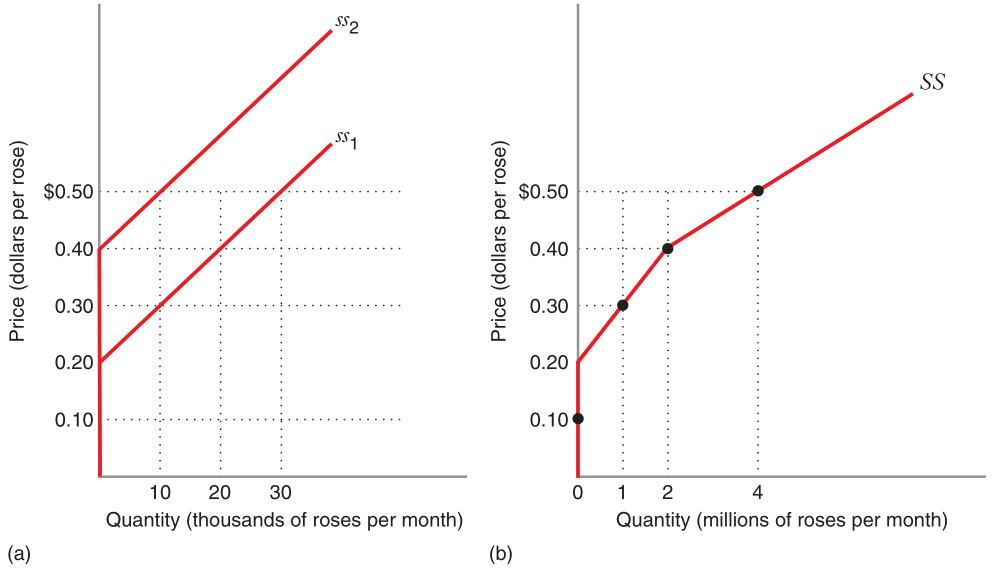
\includegraphics[width=260px]{figures/fig9_6.jpg}
  \end{figure}
\end{frame}

\begin{frame}{Short-Run Perfectly Competitive Equilibrium}
  Now that we have a market supply curve, we can find the \textbf{short-run perfectly competitive equilibrium}.

  \begin{itemize}
    \item That is, the price at which quantity supplied equals quantity demanded.
  \end{itemize}

  \bigskip
  \begin{figure}
    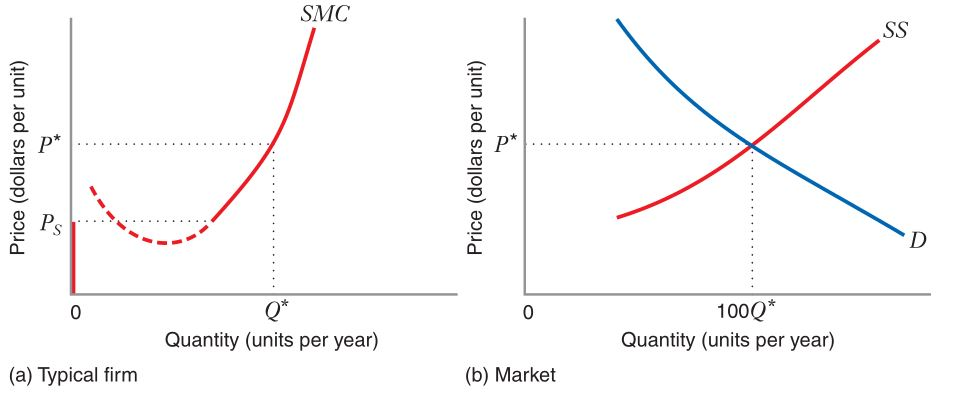
\includegraphics[width=280px]{figures/fig9_8.jpg}
  \end{figure}
\end{frame}

\begin{frame}{\bgCoral{Try It Yourself}}
  Suppose that a market is made up of 300 identical firms, each with short-run total cost curve $STC(Q) = 0.1 + 150Q^2$, and corresponding marginal cost $SMC(Q)=300Q$ and average variable cost $AVC(Q)=150Q$. If market demand for the good is $D(P)=60-P$, find the market equilibrium, assuming that all firms will supply at any price.
\end{frame}

\begin{frame}{Comparative Statics Analysis}
  Suppose that the number of firms in a market increases (for example, suppose a large number of new oil refineries were built).

  \begin{itemize}
    \item This will shift the supply curve to the right.
    
    \item In chapter 2 we learned that if this happens, equilibrium \emph{price} will fall, and equilibrium quantity will rise.
  \end{itemize}
\end{frame}

\begin{frame}{Comparative Statics Analysis}
  \begin{figure}
    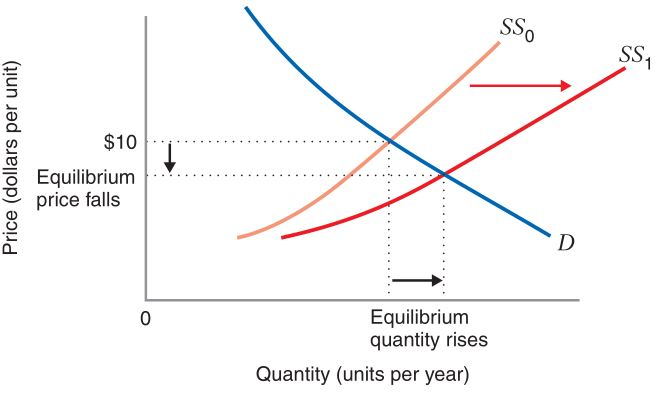
\includegraphics[width=240px]{figures/fig9_9.jpg}
  \end{figure}
\end{frame}

\begin{frame}{Comparative Statics Analysis}
  Or suppose that demand increases (maybe an economic boom means higher incomes for consumers).

  \begin{itemize}
    \item Then the market price will rise, and more units will be bought and sold.
  \end{itemize}

  \bigskip\pause 
  The magnitude of these changes depends on how responsive supply is to a change in price.

  \begin{itemize}
    \item If suppliers can't change their output level easily (inelastic supply), then price might rise by a lot (e.g. corn farmers).
    
    \item If suppliers can easily change their output level (elastic supply), then price might not rise by much, and quantity sold increases (e.g. hair salon).
  \end{itemize}
\end{frame}

\begin{frame}{Comparative Statics Analysis}
  \begin{figure}
    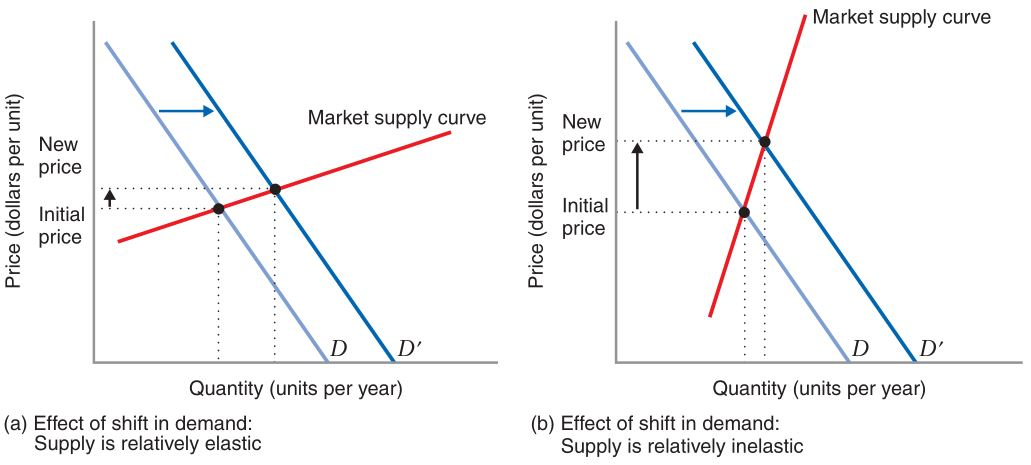
\includegraphics[width=290px]{figures/fig9_10.jpg}
  \end{figure}
\end{frame}

\begin{frame}{\bgCoral{Try It Yourself}}
  Suppose that in the Denver pizza market, the market supply curve is perfectly elastic. If people decide that pizza causes cancer, and demand falls, what will be the short-run effect on the equilibrium price and quantity?

  \medskip
  \begin{enumerate}[A)]
    \item Price increases, quantity decreases
    \item Price decreases, quantity decreases
    \item Price unchanged, quantity decreases
    \item Price unchanged, quantity increases
  \end{enumerate}
\end{frame}

\begin{frame}{Long-Run Equilibrium}
  In the short-run, new firms can't easily enter or exit the market.

  \begin{itemize}
    \item So profit might be positive or negative.
  \end{itemize}

  \medskip\pause
  In the long-run, however, firms can enter or exit, which drives profit to zero.

  \begin{itemize}
    \item If per-unit profits are positive, firms enter the market and lower the price and hence the per-unit profit margin
    \item If per-unit profits are negative, firms exit the market and raise the price and hence the per-unit profit margin
  \end{itemize}

  \medskip\pause
  Firms in the long-run can also adjust plant size (and other fixed inputs), leading to new short-run cost curves.
\end{frame}

\begin{frame}{Long-Run Equilibrium}
  \begin{figure}
    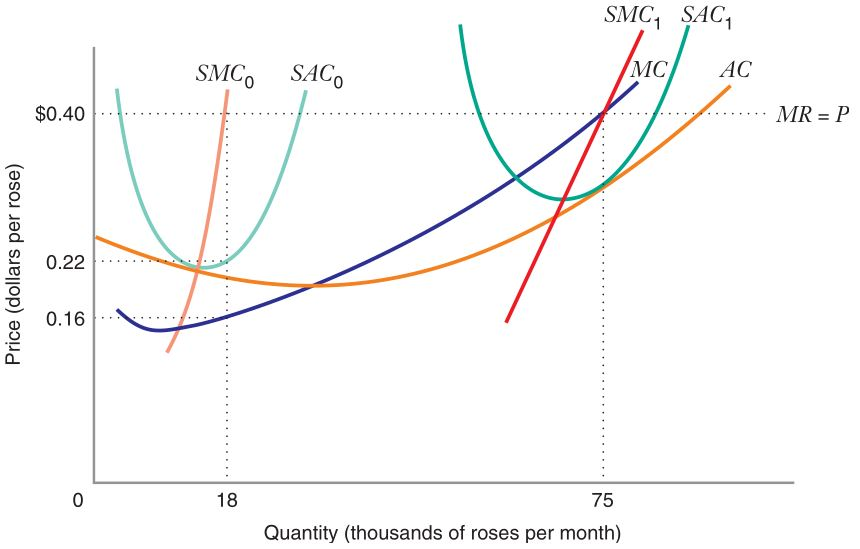
\includegraphics[width=260px]{figures/fig9_12.jpg}
  \end{figure}
\end{frame}

\begin{frame}{The Firm's Long-Run Supply Curve}
  Similar to the short run, the firm's long-run supply curve is equal to it's LRMC curve, for most prices.

  \begin{itemize}
    \item But only if the firm is earning positive profit overall ($\pi \geq 0$).
    \item That is, only if $LRAC \geq P$
  \end{itemize}

  \bigskip
  If the firm isn't earning positive profit, it will exit the market in the long run (raising the market price).
\end{frame}

\begin{frame}{The Firm's Long-Run Supply Curve}
  \begin{figure}
    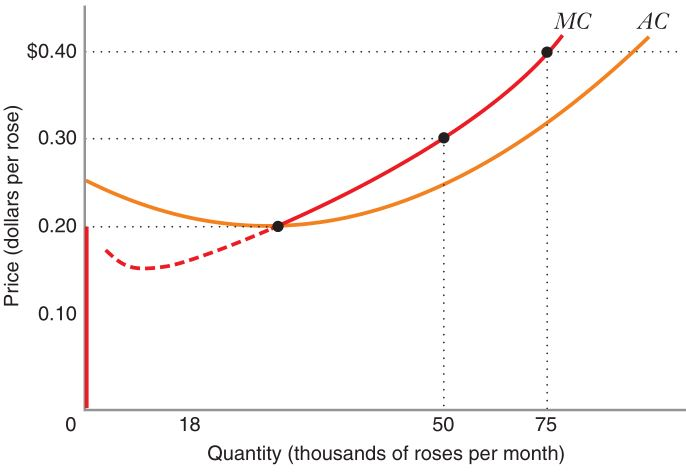
\includegraphics[width=250px]{figures/fig9_13.jpg}
  \end{figure}
\end{frame}

\begin{frame}{Long-Run Market Equilibrium}
  \begin{itemize}
    \item If per-unit profits are positive, $P^* \geq AC(Q^*)$, firms enter the market and lower the price and hence the per-unit profit margin
    \item If per-unit profits are negative, $P^* \geq AC(Q^*)$, firms exit the market and raise the price and hence the per-unit profit margin
  \end{itemize}
  
  \bigskip
  This drives long-run profits toward zero where $P^* = AC(Q^*)$.
\end{frame}

\begin{frame}{Long-Run Market Equilibrium}
  \begin{figure}
    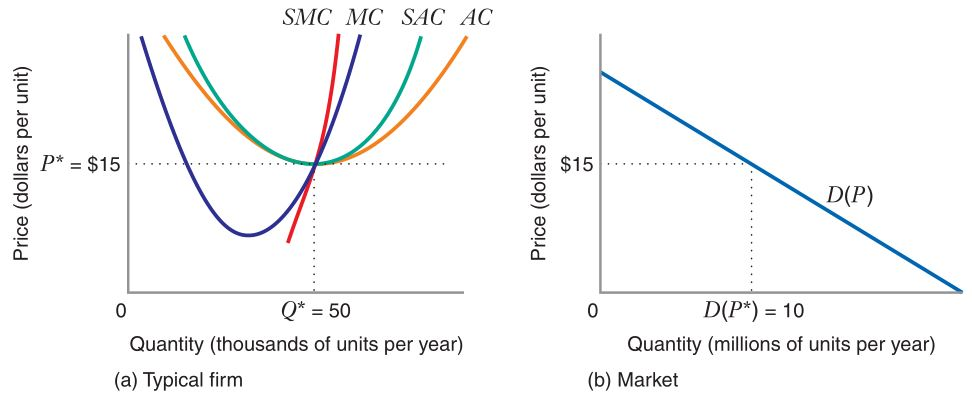
\includegraphics[width=300px]{figures/fig9_14.jpg}
  \end{figure}
\end{frame}

\begin{frame}{Long-Run Market Equilibrium}
  We can define the long-run perfectly competitive equilibrium as follows:
  
  \bigskip
  \begin{itemize}
    \item Each firm chooses $Q^*$ to maximize long-run profit, or $P^* = MC(Q^*)$ (zero profit).

    \item Each firm's economic profit is zero, or $P^* = AC(Q^*)$

    \item Market demand equals market supply at the equilibrium price, or $Q^*_D(P^*)=Q^*_S(P^*)$.
  \end{itemize}
\end{frame}

\begin{frame}{\bgCoral{Example}}
  Suppose that a market is composed of identical firms. Each firm has long-run cost curve $AC(Q) = 40 - Q + 0.01Q^2$ and corresponding marginal cost curve $MC(Q) = 40 - 2Q + 0.03Q^2$. 
  
  \bigskip
  The market demand curve is given by $D(P) = 25,000 - 1000P$. Find the long-run equilibrium quantity and market price.

  \bigskip\pause
  The first two equilibrium conditions, $P^* = MC(Q)$ and $P^* = AC(Q)$, imply that $MC(Q) = AC(Q)$. That is,

  $$
    40 - Q + 0.01Q^2 = 40 - 2Q + 0.03Q^2 \pause\implies Q^* = 50
  $$
\end{frame}

\begin{frame}{\bgCoral{Example}}
  We can plug the firm's optimal quantity in to find their $MC$, and thus, the market price.
  $$
    P^* = MC(Q^*) = 40 - 2*50 + 0.03*50^2 = 40 - 100 + 2,500 * 0.03 = 15
  $$

  \bigskip\pause
  At a price of \$15, consumer demand is given by 
  $$
    D^*(P^*) = 25,000 - 1000*15 = 10,000
  $$
\end{frame}

\begin{frame}{\bgCoral{Example}}
  Finally, we need to find the equilibrium number of firms needed to supply 10,000 units. That is,
  \pause
  $$
    Q^*_D(P^*) = n^* Q_{firm}^*(P^*) \pause \implies n^* = 10,000 / 50 = 200.
  $$
\end{frame}

\begin{frame}{Long-Run Market Equilibrium}
  Therefore, in this market, the long-run equilibrium can be defined as follows:
  \begin{align*}
    P^*        & =15  \\
    Q^*_{firm} & =50  \\
    n^*        & =200
  \end{align*}
\end{frame}

\begin{frame}{\bgCoral{Try It Yourself}}
  Suppose that consumer demand has increased, such that $D(P^*)=30,000-1,000P^*$. Find the new long-run equilibrium number of firms.
\end{frame}

\begin{frame}{}
\end{frame}

\begin{frame}{Long-Run Market Supply Curve}
  The \textbf{long-run market supply (LS) curve} tells us the total quantity of output that will be supplied at every price, assuming that all long-run adjustments have taken place.

  \begin{itemize}
    \item In other words, the long-run market supply curve traces the equilibria that result from increases in demand.
  \end{itemize}
\end{frame}

\begin{frame}{Long-Run Market Supply Curve}
  \begin{figure}
    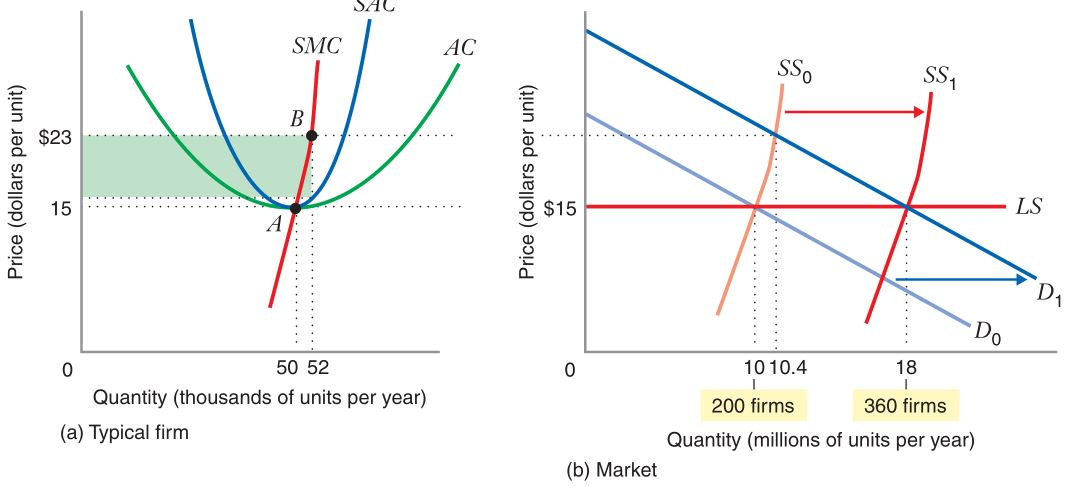
\includegraphics[width=300px]{figures/fig9_15.jpg}
  \end{figure}
\end{frame}

\begin{frame}{Constant-, Increasing-, and Decreasing-Cost Industries}
  In the previous section, we assumed that new entry doesn't affect the price of inputs.

  \bigskip
  This may be the case when an industry's demand for an input is a small part of overall demand for that input (i.e. unskilled labor, electricity, etc...)
  
  \begin{itemize}
    \item When changes in an industry's output have no effect on input prices, we call it a \textbf{constant-cost industry}.
  \end{itemize}
  
  \bigskip\pause
  However, when expansion of an industry increases the price of an input, it is an \textbf{increasing-cost industry}.
  \begin{itemize}
    \item If an industry uses \textbf{industry-specific inputs}, they are likely to be an increasing-cost industry (e.g pharmacists).
  \end{itemize}
\end{frame}

\begin{frame}{Constant-, Increasing-, and Decreasing-Cost Industries}
  When more firms enter in an increasing-cost industry, marginal costs increase for all firms in the industry.

  \begin{itemize}
    \item It costs a firm more to produce a given quantity than before.
    
    \item Thus, minimum average cost increases.
  \end{itemize}

  \bigskip
  As before, firms continue to enter until $P=\min(AC)$.

  \begin{itemize}
    \item But now $\min(AC)$ is greater than before, so the long-run equilibrium price has gone up.
    
    \item =Thus, the long-run supply curve is upward sloping.
  \end{itemize}

\end{frame}

\begin{frame}{Constant-, Increasing-, and Decreasing-Cost Industries}
  \begin{figure}
    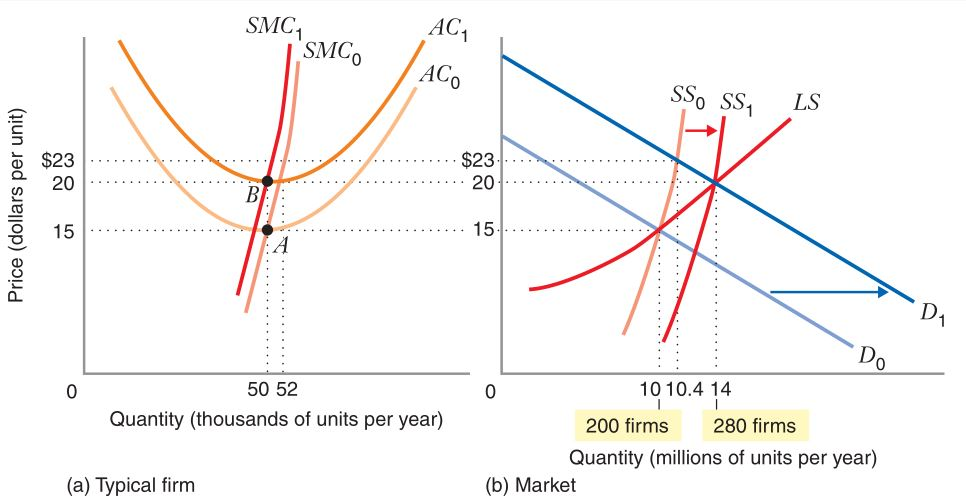
\includegraphics[width=280px]{figures/fig9_18.jpg}
  \end{figure}
\end{frame}

\begin{frame}{Constant-, Increasing-, and Decreasing-Cost Industries}
  For other industries, input prices may decrease as industry output increases.

  \begin{itemize}
    \item This can be the case if the input producers can take advantage of economies of scale (computer chips, for example).
  \end{itemize}

  \bigskip
  In this case, as firms enter, marginal costs fall for individual firms.

  \begin{itemize}
    \item And in the long-run, the price settles at the new, lower minimum average cost.
    
    \item Thus, the long-run supply curve is downward-sloping.
  \end{itemize}

\end{frame}

\begin{frame}{Constant-, Increasing-, and Decreasing-Cost Industries}
  \begin{figure}
    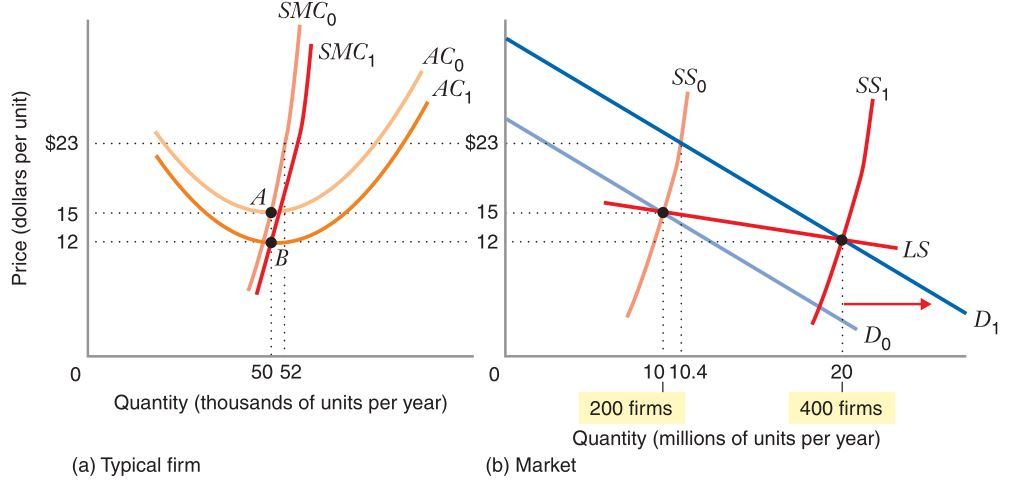
\includegraphics[width=280px]{figures/fig9_19.jpg}
  \end{figure}
\end{frame}

\begin{frame}{Producer Surplus}
  When a firm sells a product, they often sell some of the units at a higher price than they would have been \textit{willing to} sell them at.

  \bigskip
  This difference is called \textbf{producer surplus}.

  \begin{itemize}
    \item Graphically, it is the area of the supply and demand graph below the market price, but above the firm's supply curve.
    
    \item It is analogous to consumer surplus in consumer theory.
  \end{itemize}

\end{frame}

\begin{frame}{Producer Surplus}
  What if a firm faces a fixed cost in the long-run (e.g. rent and machinery)?

  \begin{itemize}
    \item Then below some price, they may not be willing to supply any quantity below a certain price.
    
    \item Below this shutdown price, consumer surplus would be zero (as the firm would not supply any of the good).
  \end{itemize}

  Some markets don't exist even though there is potential demand for it(!)
\end{frame}

\begin{frame}{\bgCoral{Try It Yourself}}
  Suppose that the market supply curve for milk is given by $Q = 60P$ (assume that there are no fixed costs), where $Q$ is the quantity of milk sold per month (measured in thousands of gallons) when the price is $P$ dollars per gallon. What is the producer surplus when the price of milk is \$3 per gallon?
\end{frame}

\end{document}
